% Theoretical Background (Priyanshu)
% Project numbers come from reports/best_params.json, reports/results.csv, reports/tuning_*.csv,
% reports/ablation.csv, notebooks/01_eda.ipynb, notebooks/02_evaluation.ipynb and src/*.py.
% Full derivations are in sections/appendix.tex. Uses \keyeq and projectbox from main.tex.

\section{Theoretical Background}
\label{sec:theory}

This section gives the theory behind four choices in our pipeline (Fig.~\ref{fig:pipeline}):
gradient-boosted trees, class weighting, PR AUC as the main metric, and why tuning stops helping. The
main results are stated here, and the full derivations are given in Appendix~\ref{app:derivations}.

% =============================================================================================
\subsection{Gradient boosting and second-order splits}
\label{sec:theory_gb}

Gradient boosting~\cite{friedman2001} builds a model as a sum of regression trees, adding one tree $f_m$
at a time and shrinking each by a learning rate $\eta$:
\begin{equation}
F_m(\mathbf{x}) = F_{m-1}(\mathbf{x}) + \eta\, f_m(\mathbf{x}) .
\label{eq:additive}
\end{equation}
The score $F$ is a log-odds, and the predicted probability is $p = \sigma(F) = 1/(1+e^{-F})$.
XGBoost~\cite{chen2016} chooses each tree by minimising a loss plus a penalty on tree complexity, where
$T$ is the number of leaves and $w_j$ the value of leaf $j$:
\begin{align}
\mathcal{L} &= \sum_{i=1}^{n} l(y_i, \hat{y}_i) + \sum_{k} \Omega(f_k), \label{eq:objective}\\
\Omega(f) &= \gamma T + \tfrac{1}{2}\lambda \textstyle\sum_{j} w_j^2 . \label{eq:omega}
\end{align}

\textbf{Second-order step.} At step $m$ the loss is expanded to second order around the current
prediction. With gradients $g_i$ and Hessians $h_i$ of the loss, which for log loss are
(Appendix~\ref{app:grad})
\begin{equation}
g_i = p_i - y_i, \qquad h_i = p_i(1-p_i),
\label{eq:gh}
\end{equation}
and with $G_j$ and $H_j$ the sums of $g_i$ and $h_i$ over the rows in leaf $j$, the objective becomes
one quadratic per leaf:
\begin{equation}
\mathcal{L}^{(m)} \approx \sum_{j=1}^{T} \Big[ G_j w_j + \tfrac{1}{2}(H_j + \lambda)\, w_j^2 \Big] + \gamma T .
\label{eq:leafsum}
\end{equation}

\textbf{Leaf values and split gain.} Setting the derivative with respect to $w_j$ to zero,
$G_j + (H_j+\lambda)\,w_j = 0$, gives the optimal leaf value and, substituted back, the lowest loss for
a given tree structure:
\begin{equation}
\keyeq{w_j^\ast = -\frac{G_j}{H_j + \lambda}}, \qquad
\mathcal{L}^{\ast} = -\frac{1}{2} \sum_{j=1}^{T} \frac{G_j^2}{H_j + \lambda} + \gamma T .
\label{eq:leafweight}
\end{equation}
Each leaf therefore takes one Newton step, the gradient divided by the curvature plus $\lambda$.
Splitting a leaf into a left part $L$ and a right part $R$ changes $\mathcal{L}^\ast$ by
\begin{multline}
\text{Gain} = \frac{1}{2}\left[ \frac{G_L^2}{H_L + \lambda} + \frac{G_R^2}{H_R + \lambda} \right. \\
\left. - \frac{(G_L + G_R)^2}{H_L + H_R + \lambda} \right] - \gamma .
\label{eq:gain}
\end{multline}
Trees are grown greedily, and a split is kept only if its gain is positive (Fig.~\ref{fig:th_split}).
So $\gamma$ is the minimum loss reduction that pays for a new leaf, and $\lambda$ shrinks leaf values
toward zero, most strongly in leaves with a small Hessian sum.

\begin{figure}[t]
\centering
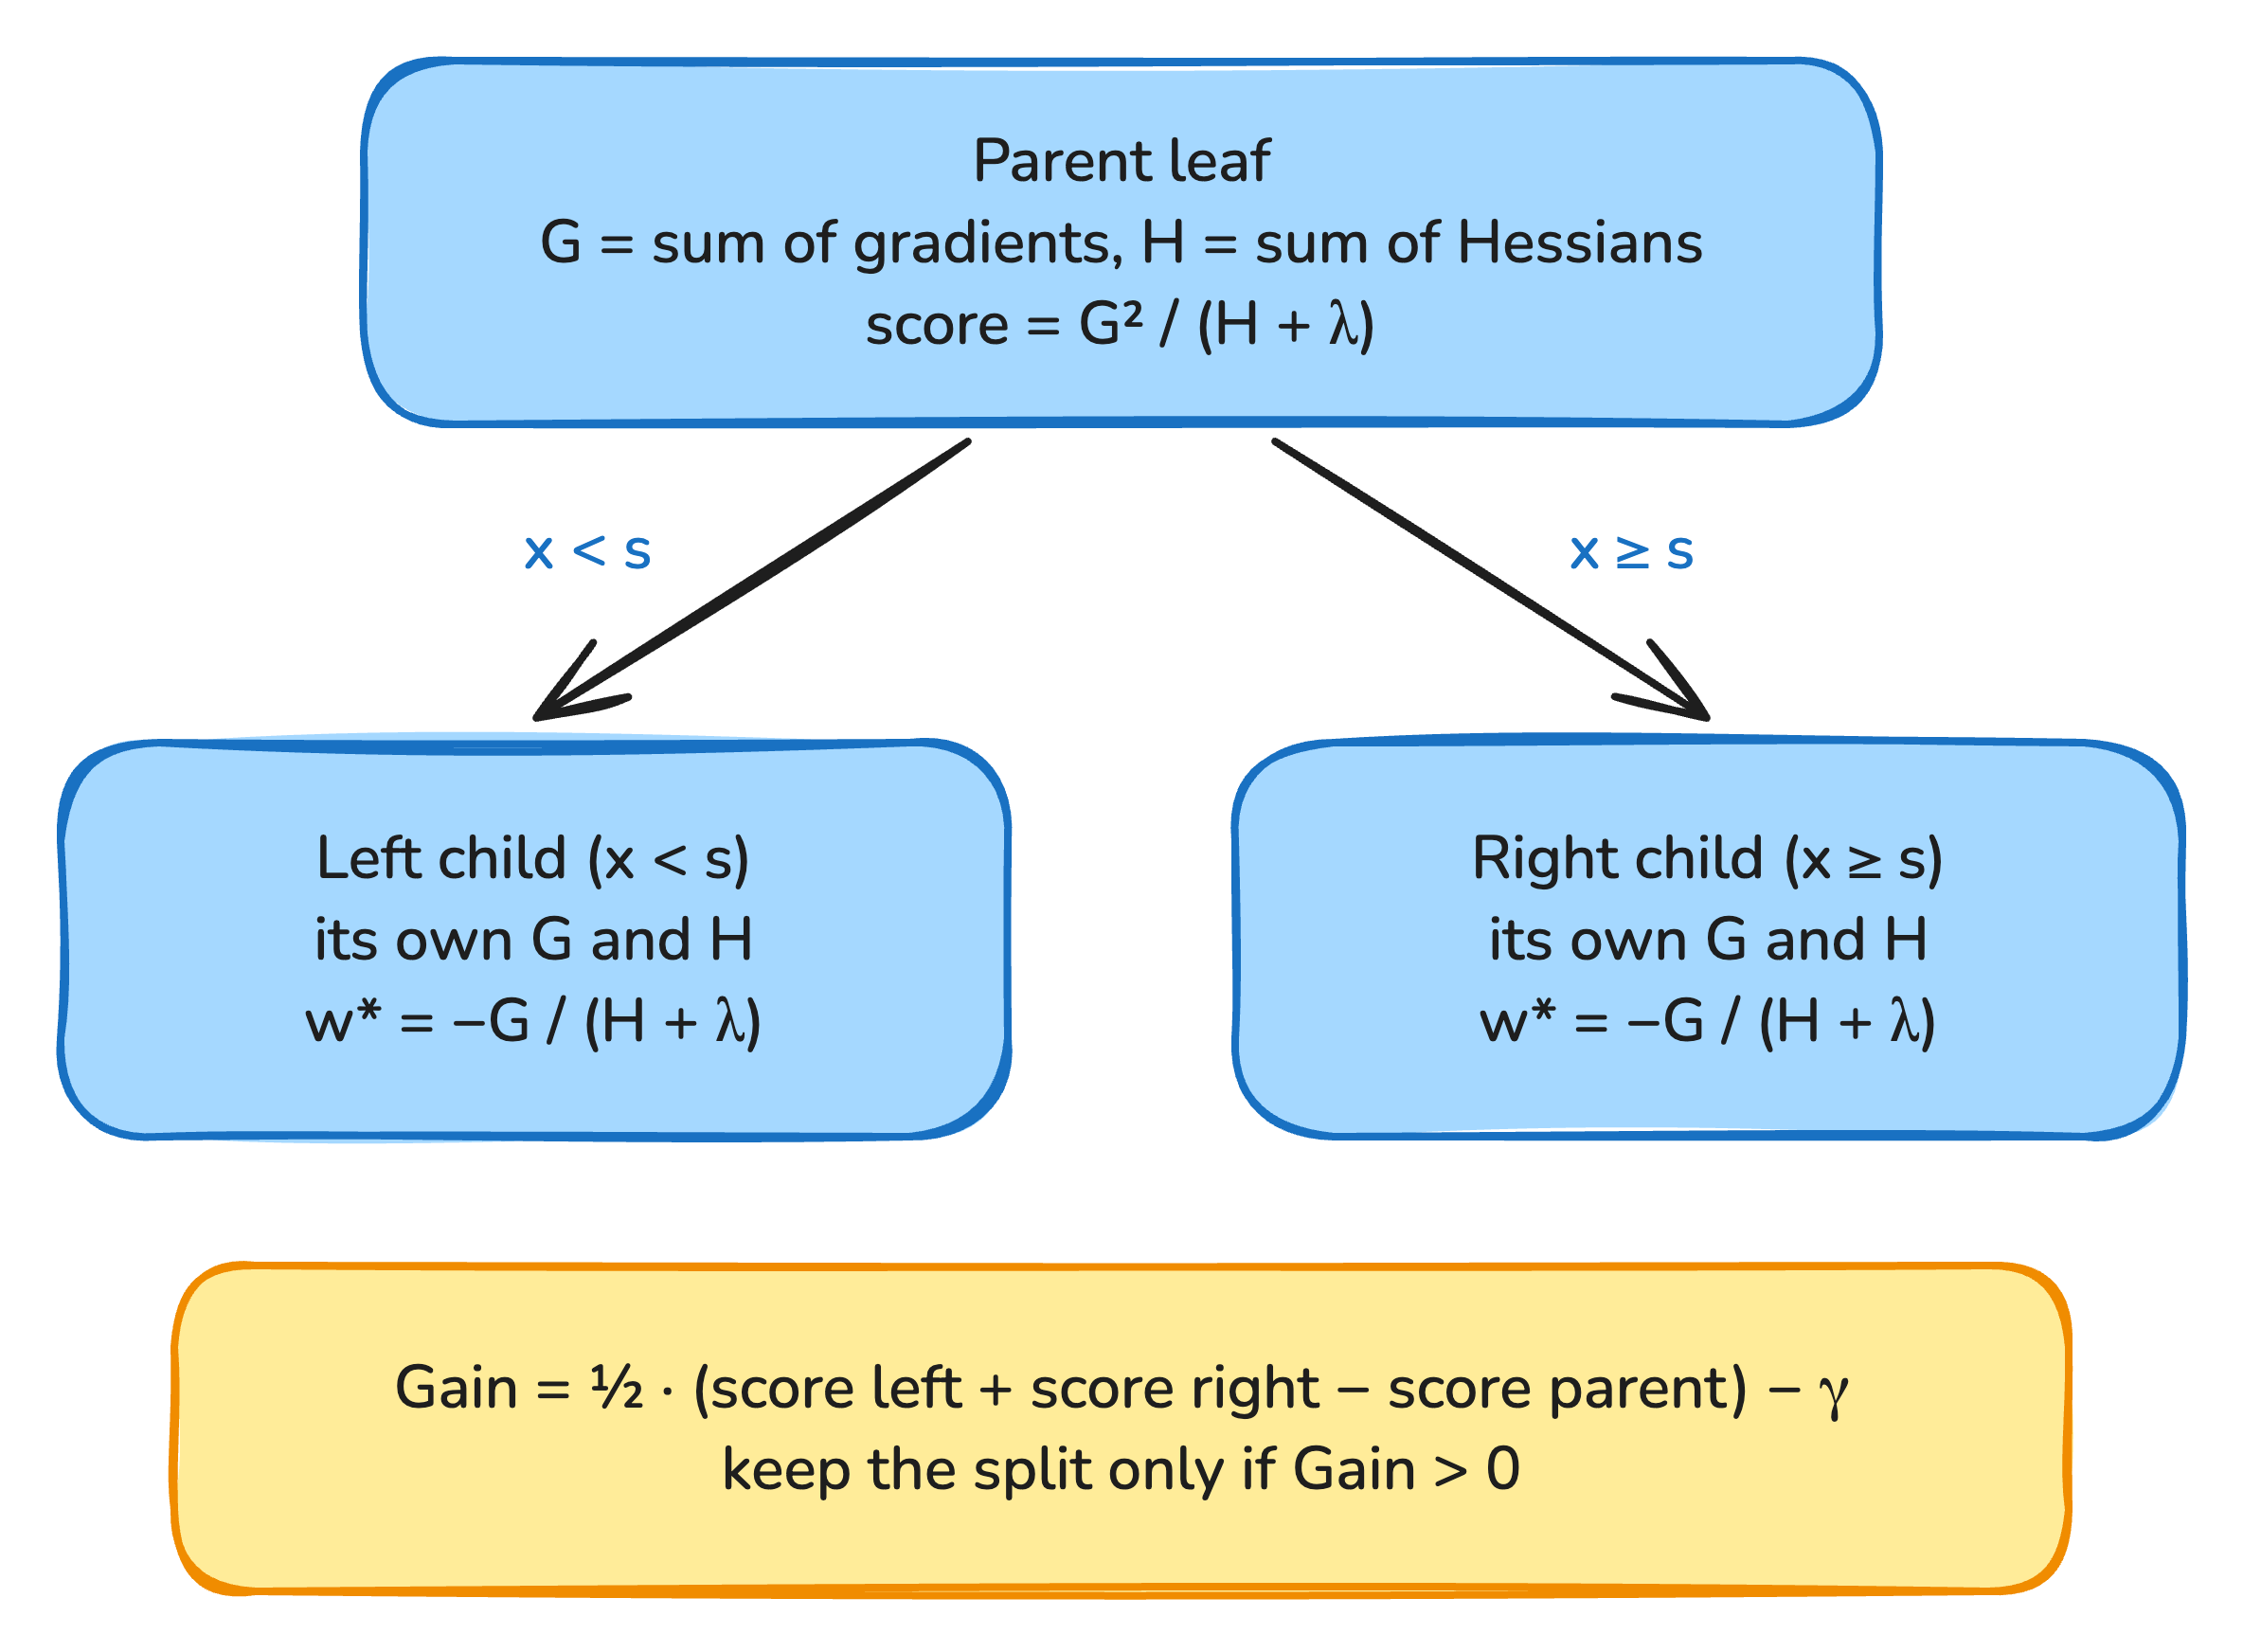
\includegraphics[width=0.92\columnwidth]{figures/th_split.png}
\caption{One split in XGBoost. Each child gets the value $w^\ast$ of (\ref{eq:leafweight}); the split is
kept only if the gain (\ref{eq:gain}) is positive.}
\label{fig:th_split}
\end{figure}

\textbf{LightGBM.} LightGBM~\cite{ke2017} minimises the same kind of objective but differs in four ways.
It bins each feature into a histogram, so split search scans bins instead of sorted values. It grows
trees leaf-wise, always splitting the leaf with the largest loss reduction, so tree size is set by
\texttt{num\_leaves} rather than depth. It can sample rows by gradient size (GOSS). It bundles sparse
features that are rarely non-zero together (EFB).

\textbf{Early stopping.} Each added tree lowers the training loss, so the number of trees sets how
closely the ensemble fits the training table. Stopping when the held-out score no longer improves
chooses that number on data the trees were not fitted to, and in that way limits overfitting.

\begin{projectbox}
Table~\ref{tab:hyper} maps each symbol to its parameter and selected value (search space in
Table~\ref{tab:space}). In XGBoost, \texttt{min\_child\_weight} is the smallest $H_j$ allowed in a child.
By (\ref{eq:gh}) a no-fire row has $h \le 0.25$ and a fire row, weighted by 5, has $h \le 1.25$, so our
value of 1 is a weak constraint. The other two penalties are strong: $\gamma = 1$ is the largest value
searched, and $\lambda = 7.22$ lies near the top of $[0.1, 10]$. XGBoost uses histogram binning
(\texttt{tree\_method=hist}). LightGBM grows leaf-wise with 15 leaves and uses plain bagging, not GOSS.
Both models stop after 50 rounds without improvement in eval PR AUC, keeping 216 and 294 of at most
1\,000 trees. We stop on PR AUC rather than log loss because the 1:5 training table shifts the
probabilities (Section~\ref{sec:theory_imb}). On log loss, our LightGBM runs stopped after a single tree
(\texttt{src/train.py}).
\end{projectbox}

\begin{table}[t]
\centering
\caption{Boosting symbols and our selected values (\texttt{reports/best\_params.json}).}
\label{tab:hyper}
\small
\setlength{\tabcolsep}{4pt}
\renewcommand{\arraystretch}{1.12}
\begin{tabular}{l>{\raggedright\arraybackslash}p{2.75cm}rr}
\toprule
\rowcolor{tblhead}
\textbf{Symbol} & \textbf{Meaning} & \textbf{XGBoost} & \textbf{LightGBM} \\
\midrule
$\lambda$ & L2 penalty on leaf values & 7.22 & 0.28 \\
$\gamma$ & minimum gain per split & 1 & 1 \\
$\eta$ & learning rate & 0.026 & 0.058 \\
$\min H_j$ & minimum leaf size & $H_j \ge 1$ & 500 rows \\
- & tree size & depth 6 & 15 leaves \\
- & rows per tree & 0.73 & 0.98 \\
- & features per tree & 0.63 & 0.88 \\
$w$ & weight on fire rows & 5.0 & 5.0 \\
$M$ & trees after early stopping & 216 & 294 \\
\bottomrule
\end{tabular}
\end{table}

% =============================================================================================
\subsection{Class imbalance and class weighting}
\label{sec:theory_imb}

Next-day fire covers 1.10\% of labelled training pixels, about 90 no-fire pixels per fire pixel. Left
uncorrected, no-fire rows dominate $G_j$ and $H_j$ in every leaf. The two standard corrections are to
subsample negatives and to weight positives.

\textbf{Weighting acts like duplication.} With weight $w$ on positives, the log loss and the gradient and
Hessian of a positive row become (Appendix~\ref{app:grad})
\begin{gather}
l_w = -\big[\, w\, y \log p + (1 - y) \log(1-p) \,\big], \label{eq:weighted_ll}\\
g_i = w\,(p_i - 1), \qquad h_i = w\,p_i(1-p_i). \label{eq:weighted_gh}
\end{gather}
Both are $w$ times their unweighted values. Trees see the data only through $G$ and $H$, so a weighted
positive acts exactly like $w$ copies of the same row.

\textbf{Both corrections shift the probabilities.} Keeping a share $r$ of the negatives and weighting
positives by $w$ changes the class prior seen by the loss but not the feature distribution within each
class. By Bayes' rule (Appendix~\ref{app:shift}), the probability $p'$ learned in training and the true
probability $p$ differ by a constant factor in their odds:
\begin{equation}
\keyeq{\frac{p'}{1-p'} = \frac{w}{r}\cdot\frac{p}{1-p}}
\label{eq:prior_shift}
\end{equation}
Solving for $p$ maps a model score back to the true scale:
\begin{equation}
p = \frac{p'}{p' + (w/r)(1-p')} .
\label{eq:inverse_shift}
\end{equation}
The map is strictly increasing, so the order of pixels is unchanged. Ranking metrics (PR AUC, ROC AUC,
recall at a fixed FPR) are unaffected, but a fixed threshold must be chosen on data with the true class
ratio.

\textbf{Focal loss.} Lin et al.~\cite{lin2017} reshape the loss instead of the data. With $p_t = p$ for
positives and $1-p$ for negatives,
\begin{equation}
\mathrm{FL}(p_t) = -\alpha_t (1 - p_t)^{\gamma_f} \log p_t ,
\label{eq:focal}
\end{equation}
where $\gamma_f = 2$ and $\alpha = 0.25$ worked best in their experiments. The factor $(1-p_t)^{\gamma_f}$
is close to zero for well-classified rows, so easy negatives contribute little. With $\gamma_f = 0$ the
loss reduces to (\ref{eq:weighted_ll}).

\begin{figure}[t]
\centering
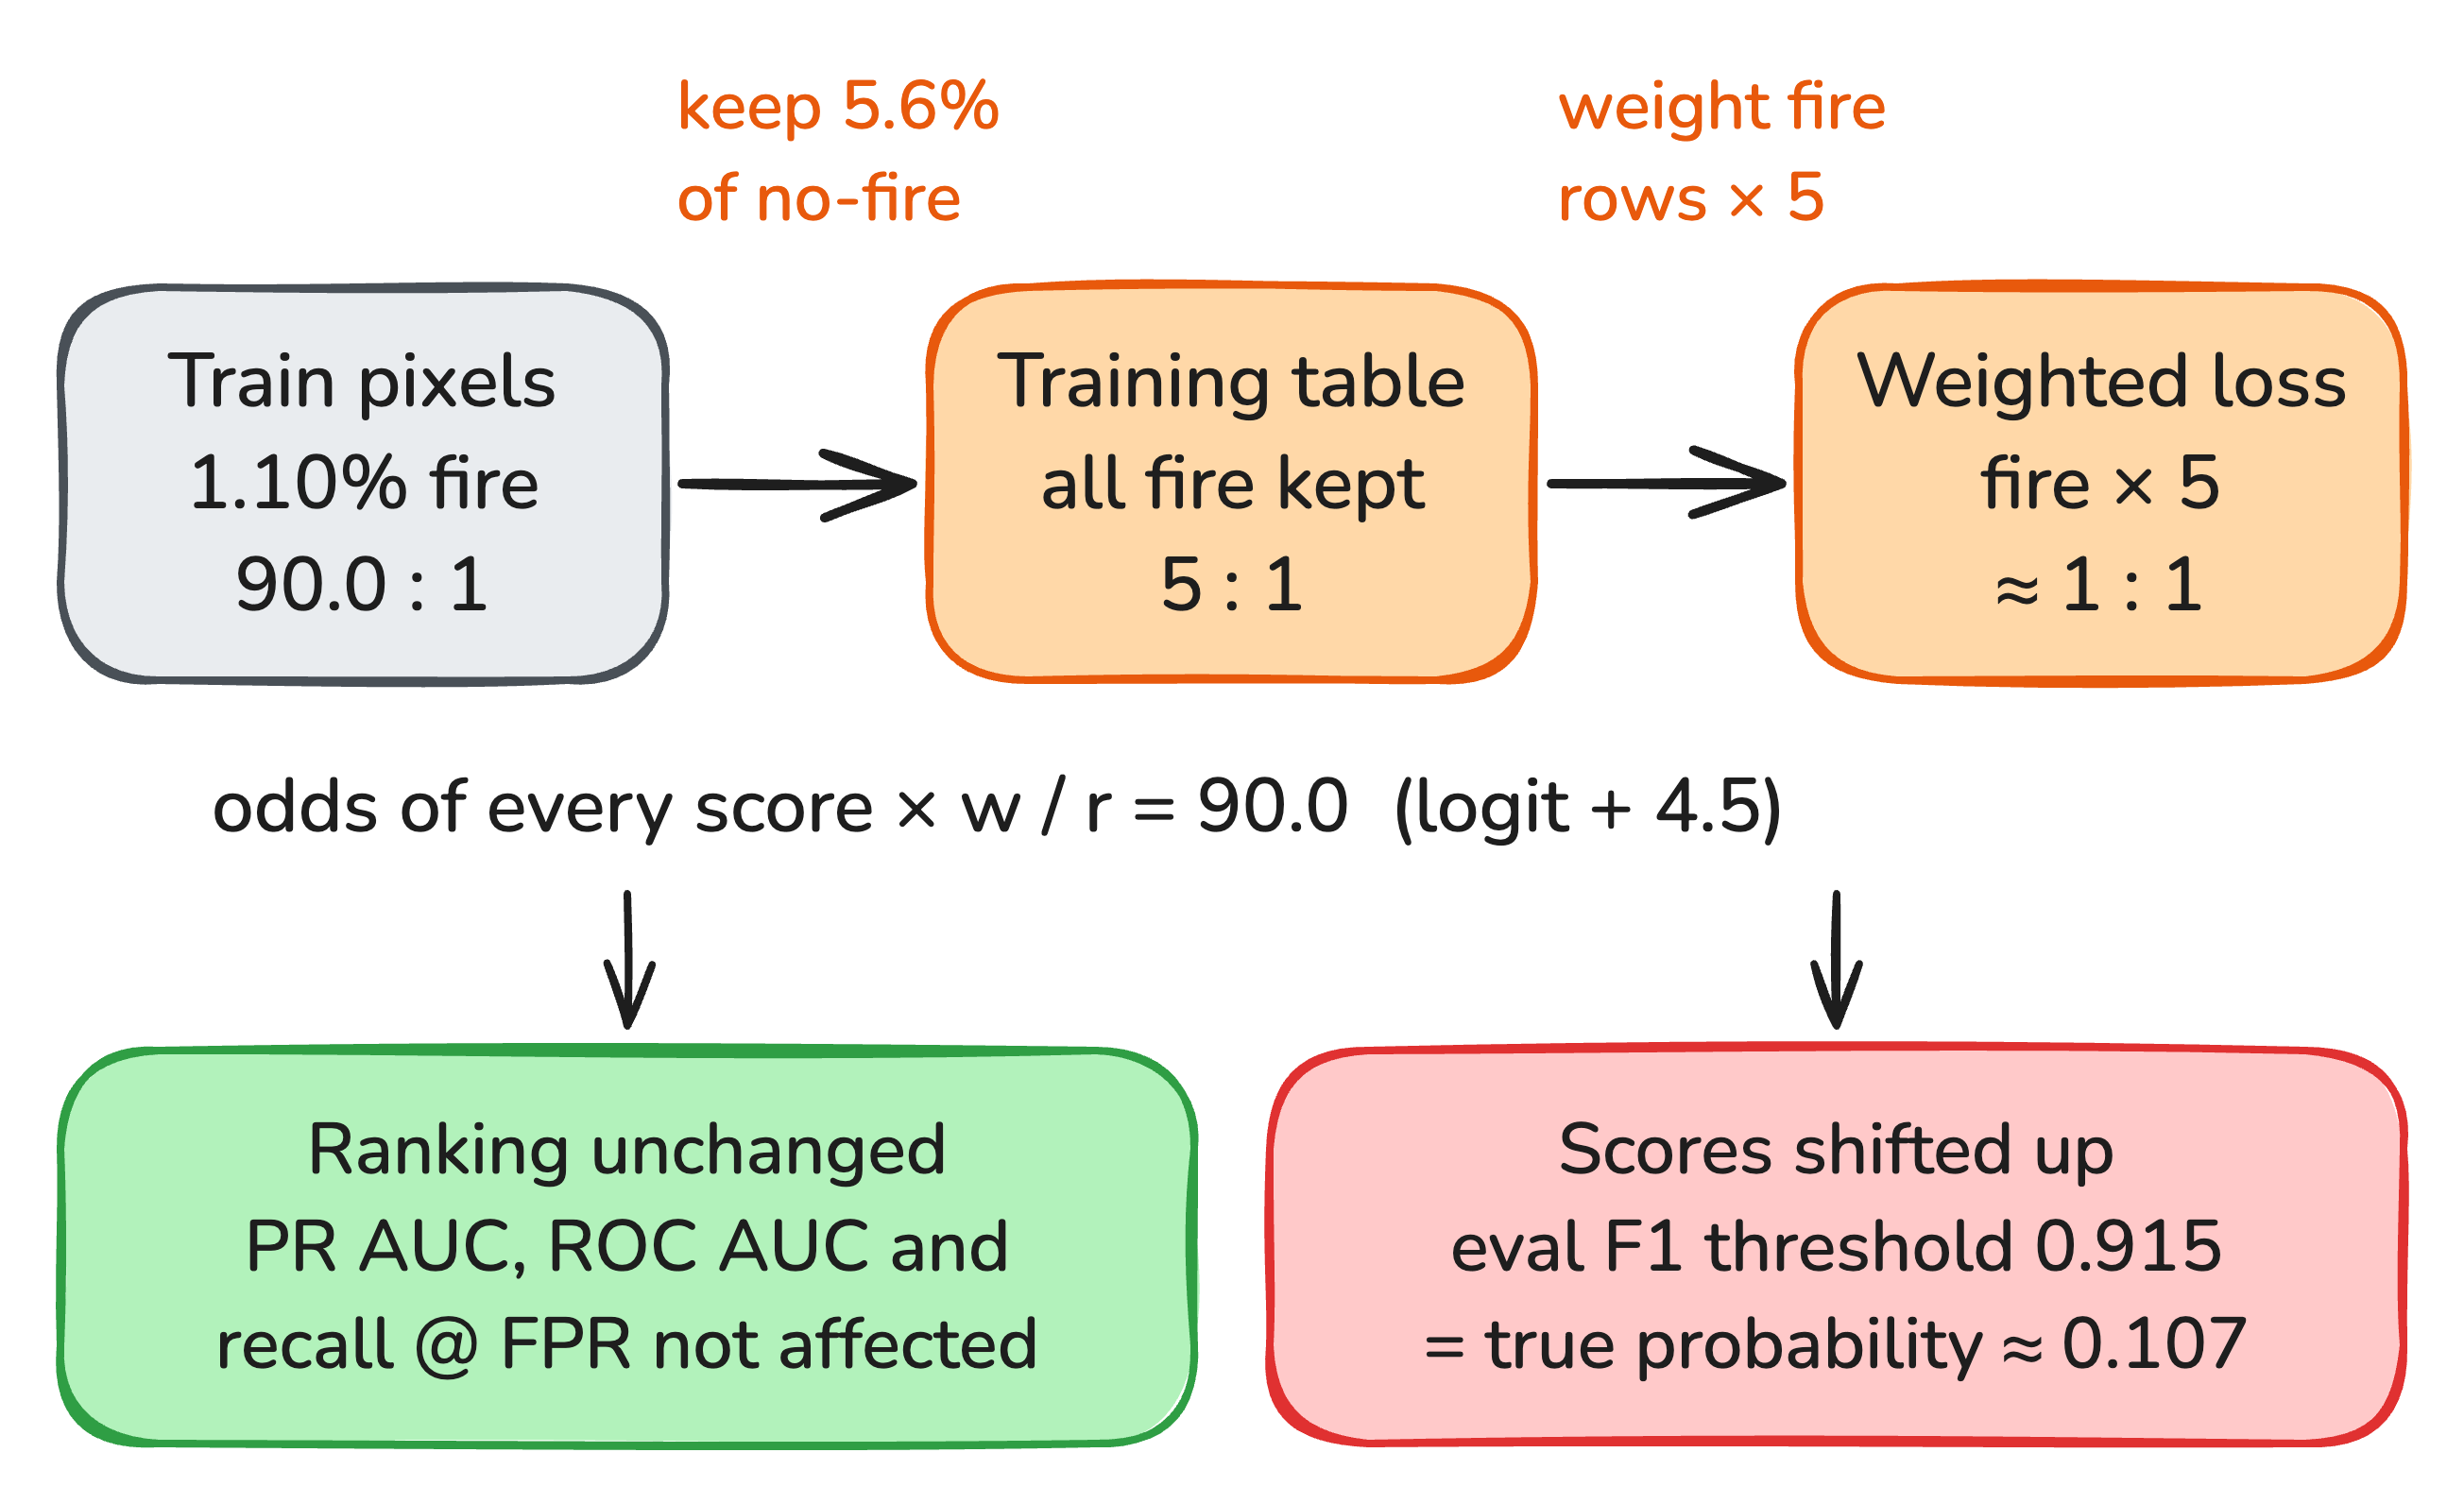
\includegraphics[width=\columnwidth]{figures/th_imbalance.png}
\caption{Subsampling and weighting turn a 90:1 problem into a balanced one and shift every score, by
(\ref{eq:prior_shift}).}
\label{fig:th_imbalance}
\end{figure}

\begin{figure}[t]
\centering
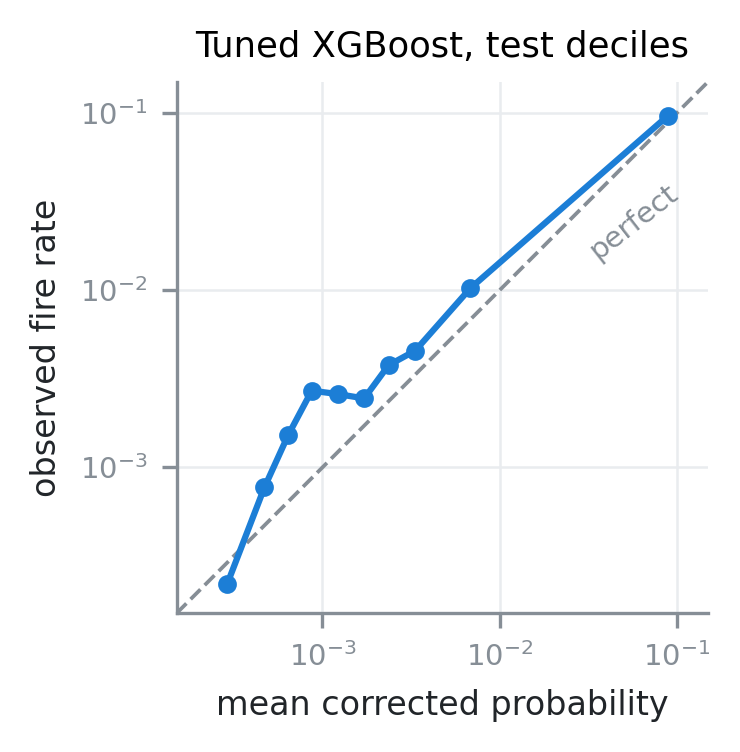
\includegraphics[width=0.68\columnwidth]{figures/th_calibration.png}
\caption{Calibration of the tuned XGBoost on test after undoing the prior shift with
(\ref{eq:inverse_shift}). Each point is one tenth of the test pixels, ordered by score; log scales.}
\label{fig:th_calibration}
\end{figure}

\begin{projectbox}
The training table keeps every fire pixel and 5 no-fire pixels per fire pixel, so $r = 5/90.0 = 0.056$,
and fire rows get $w = 5$ (\texttt{scale\_pos\_weight}). The odds are therefore multiplied by
$w/r = 90.0$, and the model trains as if the classes were balanced (Fig.~\ref{fig:th_imbalance}). This
explains the high F1 threshold of 0.915 chosen on eval: by (\ref{eq:inverse_shift}) it corresponds to a
probability of 0.107 on the true scale, while a score of 0.5 corresponds to 0.011, the training fire
rate. We checked the correction on test with a retrained copy of the model (Appendix~\ref{app:checks}).
After (\ref{eq:inverse_shift}), the mean probability is 0.0107 against an observed fire rate of 0.0125,
and in the top score decile 0.089 against 0.097 (Fig.~\ref{fig:th_calibration}). The corrected values
are therefore close to true risk and slightly low. Most of the overall gap matches the higher fire rate
of test (1.25\% against 1.10\% in train); below a corrected value of about 0.002 they are up to about 3 times
too low.

We did not use focal loss, because the boosting libraries would need it as a custom objective and weighting
already balances the loss. It is a candidate for Phase~2, where a segmentation network computes its loss
on every pixel of a patch (Huot et al.\ use a weight of 3 on fire for their CNN~\cite{huot2022}).
\end{projectbox}

% =============================================================================================
\subsection{PR AUC versus ROC AUC under imbalance}
\label{sec:theory_pr}

With $P$ fire and $N$ no-fire pixels, and TP and FP the true and false positives at a threshold,
\begin{align}
\mathrm{TPR} &= \frac{\mathrm{TP}}{P}, \qquad \mathrm{FPR} = \frac{\mathrm{FP}}{N}, \label{eq:rates}\\
\mathrm{Precision} &= \frac{\mathrm{TP}}{\mathrm{TP} + \mathrm{FP}} . \label{eq:prec_def}
\end{align}
The ROC curve plots TPR (recall) against FPR, and the PR curve plots precision against recall. Writing
precision in terms of the two rates and the prevalence $\pi = P/(P+N)$ (Appendix~\ref{app:prec}) gives
\begin{equation}
\keyeq{\mathrm{Precision} = \frac{\pi\,\mathrm{TPR}}{\pi\,\mathrm{TPR} + (1 - \pi)\,\mathrm{FPR}}}
\label{eq:precision}
\end{equation}
TPR and FPR are each computed within one class, so the ROC curve does not depend on $\pi$. Precision does:
when $\pi$ is small, $(1-\pi)\,\mathrm{FPR}$ dominates the denominator even at a small FPR.

A random classifier has ROC AUC 0.5 at any imbalance, but it also has $\mathrm{TPR} = \mathrm{FPR}$, so by
(\ref{eq:precision}) its precision is $\pi$ everywhere and its PR AUC equals the
prevalence~\cite{saito2015}. We compute PR AUC as average precision,
$\mathrm{AP} = \sum_k (R_k - R_{k-1})\, P_k$, a step sum over thresholds with recall $R_k$ and precision
$P_k$. Davis and Goadrich~\cite{davis2006} prove that a curve dominates in ROC space if and only if it
dominates in PR space, and that linear interpolation is wrong in PR space, which is why AP uses a step
sum. Saito and Rehmsmeier~\cite{saito2015} show that on imbalanced data the ROC plot can be deceptive,
while the PR plot is not.

\begin{figure}[t]
\centering
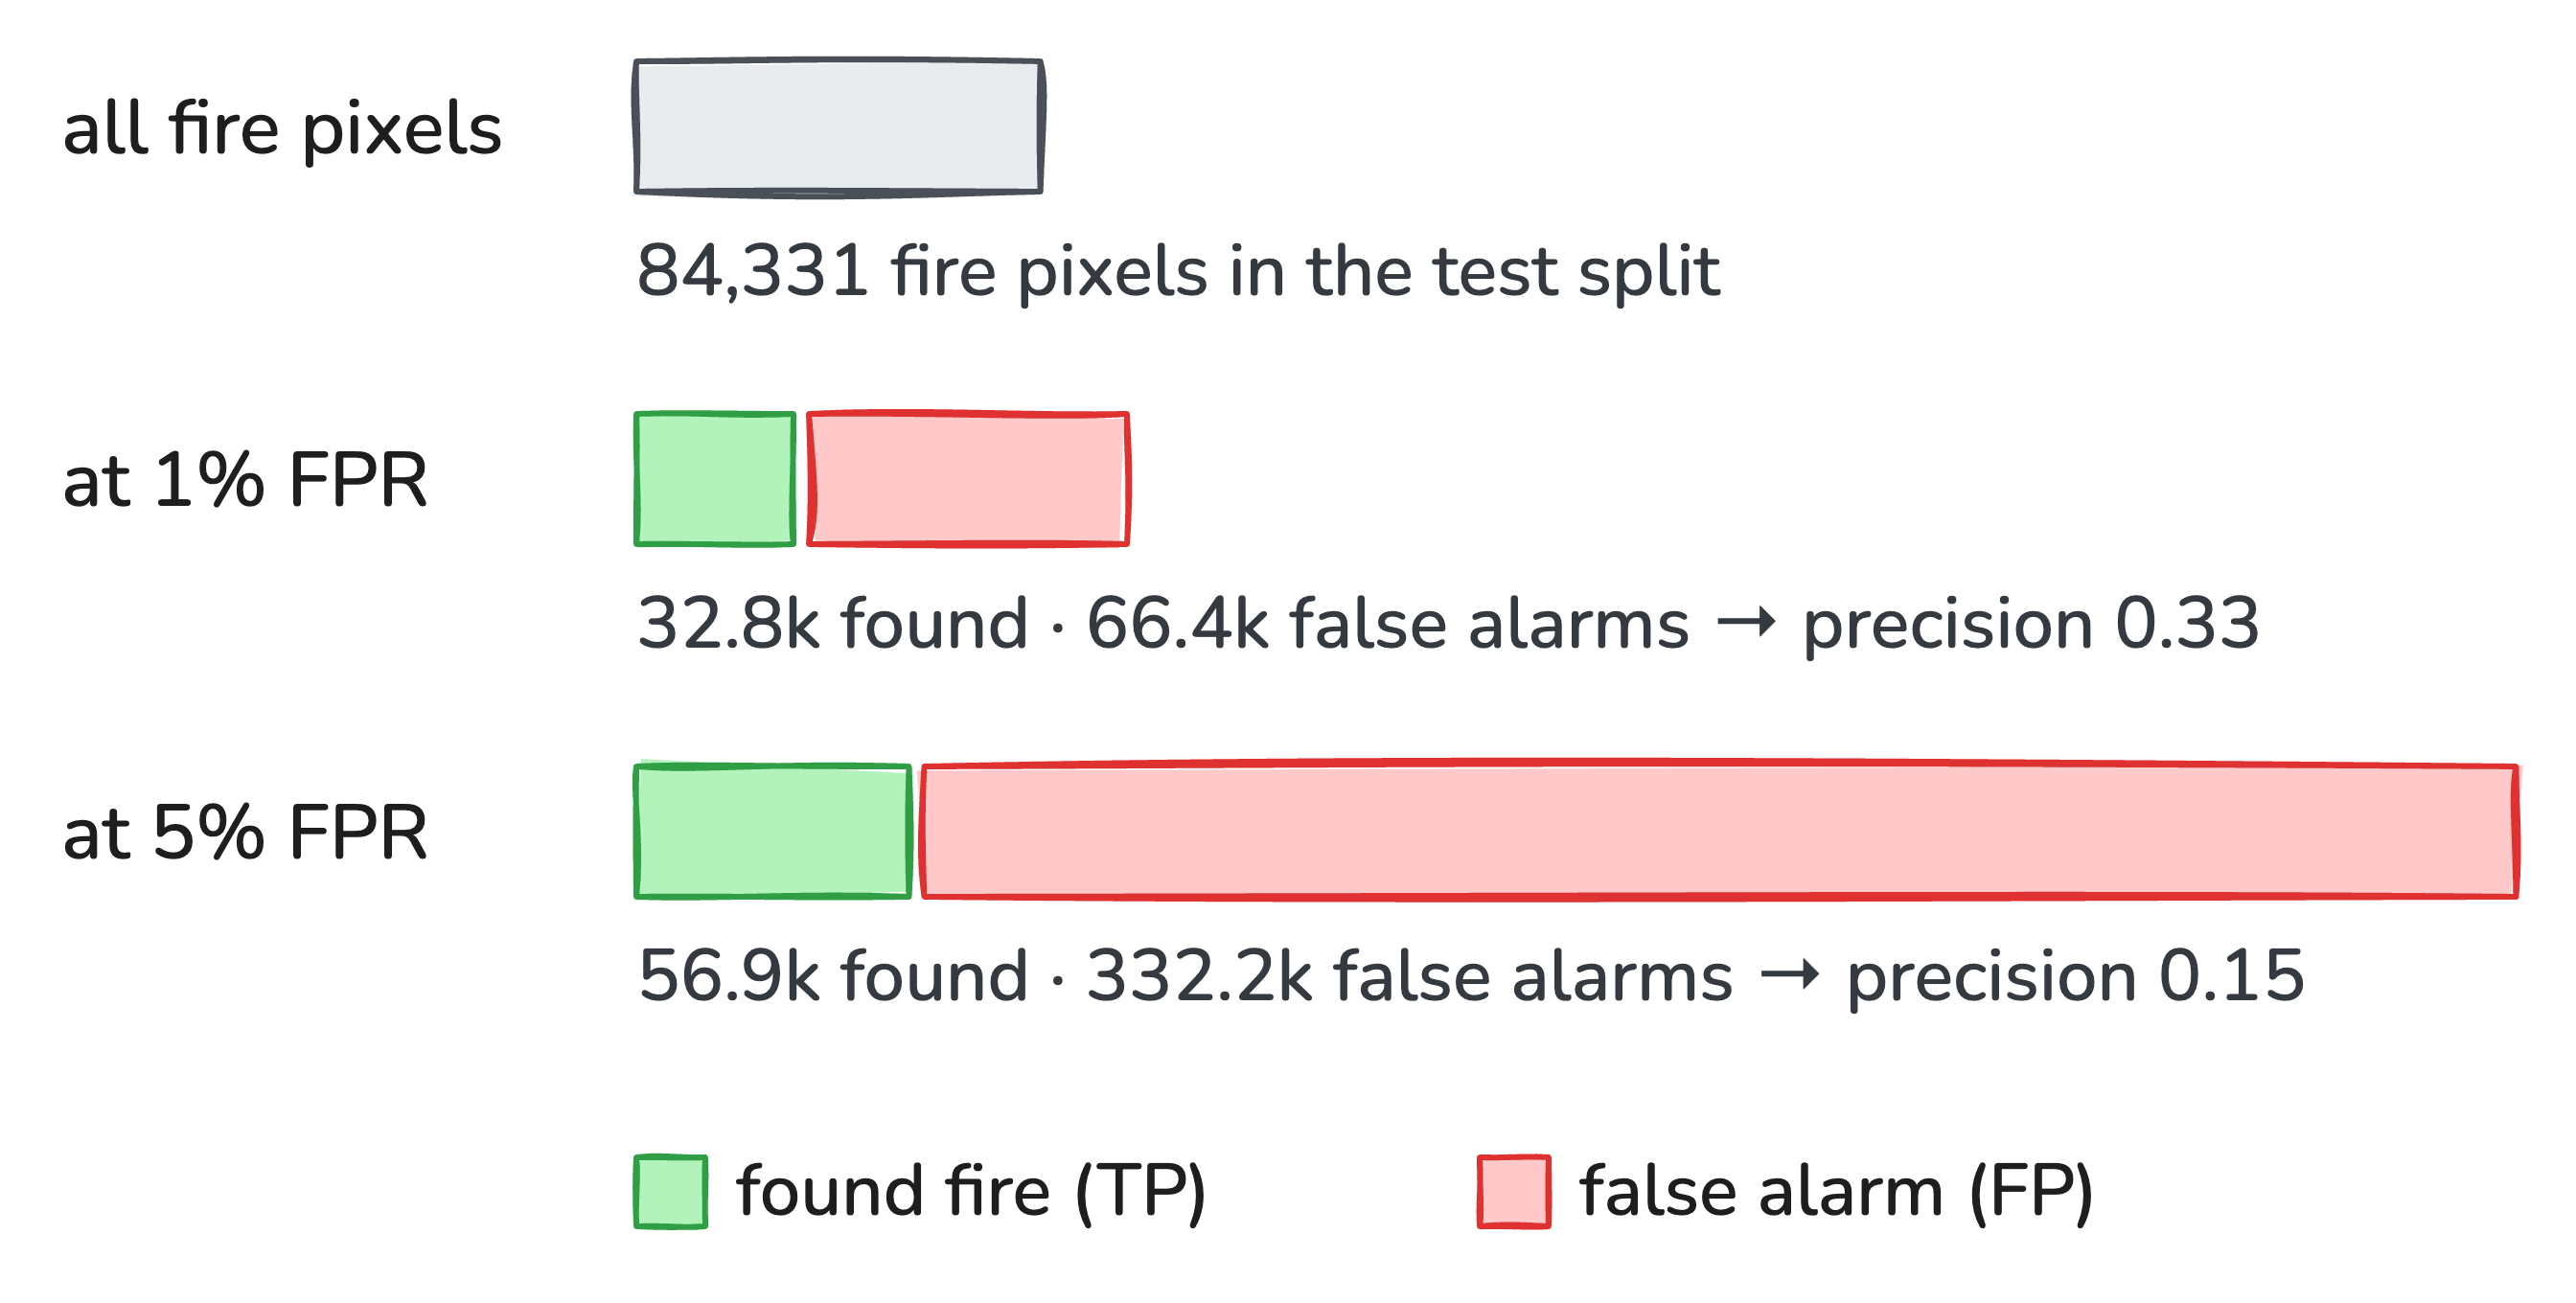
\includegraphics[width=\columnwidth]{figures/th_false_alarms.png}
\caption{Tuned XGBoost on the test split at 1\% and 5\% FPR. Box widths are proportional to pixel counts.}
\label{fig:th_false_alarms}
\end{figure}

\begin{projectbox}
Fire is 1.25\% of labelled test pixels, so a random model scores PR AUC 0.0125. Our tuned XGBoost scores
ROC AUC 0.906 but PR AUC 0.257 (Table~\ref{tab:results}). Fig.~\ref{fig:th_false_alarms} shows why the
two differ. At 1\% FPR the model finds about 32\,800 of the 84\,331 fire pixels but raises about 66\,400
false alarms, so precision is 0.33. At 5\% FPR it finds about 56\,900 against 332\,200 false alarms, a
precision of 0.15. Recall at 1\% and 5\% FPR therefore fixes the false-alarm budget an operator would
have to check. Precision, recall and F1 use the F1-optimal threshold from eval, applied unchanged to test.
Choosing it on test would overstate F1 (0.358 against 0.332).
\end{projectbox}

% =============================================================================================
\subsection{Bias-variance trade-off of tree ensembles}
\label{sec:theory_bv}

For squared loss, the expected error of a model $\hat{f}$ trained on a random training set splits into
three parts, where $f$ is the true function and $\sigma^2$ the noise variance:
\begin{equation}
\mathbb{E}\big[(y - \hat{f})^2\big] =
\underbrace{\big(\mathbb{E}\hat{f} - f\big)^2}_{\text{bias}^2}
+ \underbrace{\mathrm{Var}\,\hat{f}}_{\text{variance}}
+ \underbrace{\sigma^2}_{\text{noise}} .
\label{eq:biasvar}
\end{equation}
For log loss the split is not exactly additive, but the same reasoning applies. Bias comes from a model or
input representation that is too restricted, and variance from sensitivity to the training sample.

\textbf{Averaging trees.} For $B$ trees, each with variance $\sigma^2$ and pairwise correlation $\rho$, the
variance of their average is (Appendix~\ref{app:var})
\begin{equation}
\keyeq{\mathrm{Var}\Big(\frac{1}{B}\sum_{b=1}^{B} \hat{f}_b\Big) = \rho\,\sigma^2 + \frac{1-\rho}{B}\,\sigma^2}
\label{eq:rf_var}
\end{equation}
More trees remove only the second term, so the shared variance $\rho\sigma^2$ stays. Random
forests~\cite{breiman2001} lower $\rho$ with bootstrap samples and a random subset of features at each
split.

\textbf{Boosting.} Boosting starts from small, high-bias trees and lowers the bias step by step. Its
variance is held back by shrinkage, early stopping, tree size, minimum leaf size, the penalties $\lambda$
and $\gamma$, and row and column subsampling, which by (\ref{eq:rf_var}) also make the trees less alike.

\begin{projectbox}
Across 20 random XGBoost configurations (depth 4 to 10, learning rate 0.023 to 0.28), eval PR AUC stayed
between 0.196 and 0.207, and the 20 LightGBM configurations between 0.189 and 0.203. The settings that
trade bias against variance therefore move the score by only about 0.01. Changing the inputs moves it far
more: with the same hyperparameters, removing the fire-neighbourhood features lowers LightGBM's test PR
AUC from 0.248 to 0.048 (Table~\ref{tab:ablation}).

Learning curves (Fig.~\ref{fig:th_learning}) show where the remaining error lies. Trained on 5\% of the
training patches (0.2M rows) instead of all of them (3.9M rows), the tuned XGBoost reaches almost the
same eval PR AUC (0.204 against 0.207), and eval ROC AUC stays between 0.891 and 0.900. More data
narrows the train-eval gap in ROC AUC from 0.080 to 0.055 only by lowering the training score. More trees
do the opposite: training ROC AUC keeps rising while eval peaks at 0.898 near 270 trees and falls to
0.883 at 1000, the variance that early stopping (216 trees) avoids. An eval score that does not move with
20 times more data means the model is not limited by variance. What remains is bias from the input
representation, since each pixel sees the patch only through fixed-radius summaries, and noise the inputs
cannot explain, such as which fires will die down. This is why Phase~2 moves to a spatial model rather
than to more data or tuning.
\end{projectbox}

\begin{figure}[t]
\centering
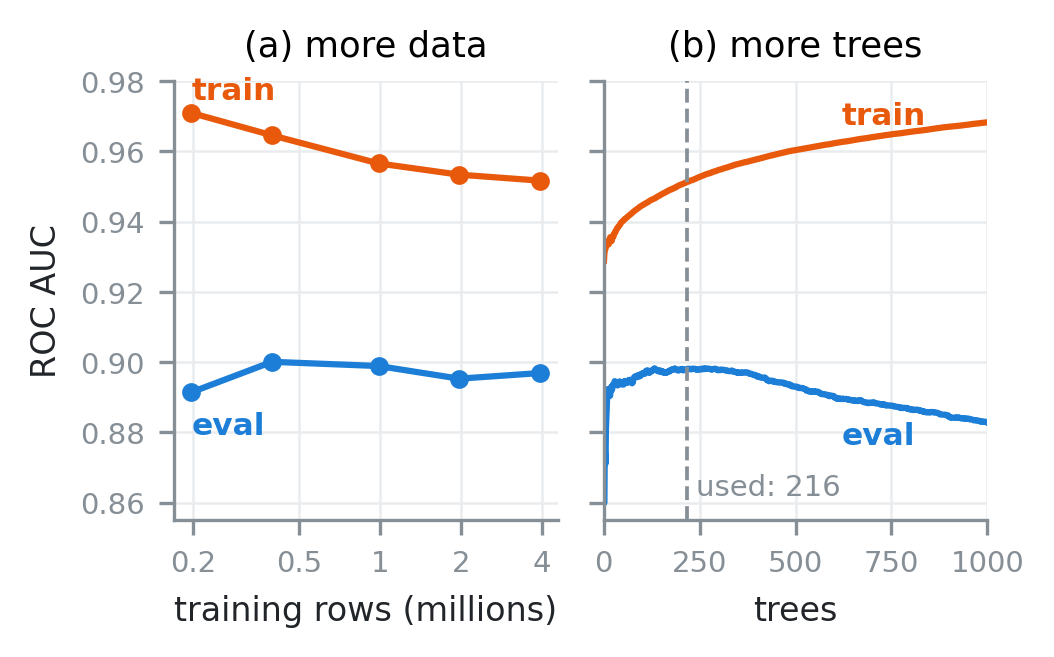
\includegraphics[width=\columnwidth]{figures/th_learning_curves.png}
\caption{Tuned XGBoost, ROC AUC on training rows and on eval. (a) Trained on 5--100\% of the training
patches. (b) Trees added without early stopping; dashed: the 216 trees used. ROC AUC is shown because the
training table is subsampled 1:5, which changes PR AUC but not ROC AUC (Section~\ref{sec:theory_pr}).}
\label{fig:th_learning}
\end{figure}
